\section{Packetization}

\subsection{Current situation in GNU Radio}
\subsubsection{GNU Radio 3.7.9}

Packet encoder and decoder blocks with limited functionality exist in GNU Radio. The \textit{Packet Encoder} and \textit{Packet Decoder} are deprecated blocks that have the following functionality:
\begin{tight_itemize}
\item Create packets with a preamble, acces code, header and a payload. The header is a double repetition of the payload length (16 bits for each field).
\item Constellations: GMSK, DBPSK, DQPSK, D8PSK, QAM8, QAM16, QAM64, QAM256
\item Modulation and pulse shaping with a given number of samples per symbol.
\end{tight_itemize}

The decoder looks for the access code and calculates the number of wrong bits. When this number is under the given threshold, it reads the header to find the payload length. Finally, it outputs the payload as a byte or float stream.

\begin{figure}[H]
    \centering
    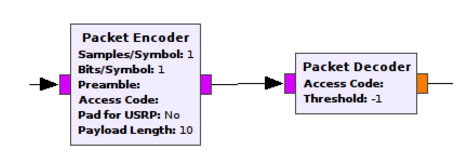
\includegraphics[width=0.6\textwidth]{img_packets/packet_encdec.png}
    \caption{Deprecated packet encoder and decoder blocks}
    \label{fig:packet_encdec}
\end{figure}

The implementation has several limitations:
\begin{tight_itemize}
\item No support for different constellations for preamble, header and payload
\item No proper support for custom header fields. The header is built as a two times the payload length.
\item Lacks flexibility: fixed payload length, pulse shaping not configurable
\item Not enough documentation and the source code is difficult to understand. For example, the output format is not specified.
\end{tight_itemize}

\subsubsection{GNU Radio 3.7.10}
New packet examples are included in this more recent version of GNU Radio. As explained in section 5.2, installing GNU Radio using the recommend way does not guarantee the latest version of GNU Radio. The existence of these packet-related example systems had been discovered late in the project and the project is developed independently.
\newpage
\subsection{Extended Packet Encoder}
\subsubsection{Requirements}
The new packet encoder implementation will limit its functionality to packetizing the incoming data stream with a preamble, header and payload and mapping these to constellation symbols. It will not do any pulse shaping or resampling.\medskip


The new packet encoder supports the following features:
\begin{tight_itemize}
\item GNU Radio's constellation objects in order to support a wide range of PSK and QAM mappings. Optional support for differential encoding.
\item Possibility to use distinct constellation types for preamble, header and payload.
\item GNU Radio's header formatter objects in order to support headers with custom lengths and fields.
\item The start of the payload data for a packet is indicated in the incoming byte stream with a tag that has the payload length as tag value.
\item Optional support for data whitening, as discussed in section 4.4.
\end{tight_itemize}


\begin{table}[H]
  \begin{center}
  \begin{tabular}{|l|l|}

    \hline
    Inputs & Outputs\\
    \hline
    \hline
    Byte stream: 1 bit/byte & Complex: mapped symbols  \\
    A tag should indicate the packet start and length & \\
    \hline

  \end{tabular}
  \end{center}
  \end{table}
   \vspace*{-0.5cm}
  \begin{table}[H]
  \begin{center}
  \begin{tabular}{|l|l|p{6cm}|}
    \hline
    Parameter name & Data type & Description\\
    \hline
    \hline
    Preamble & complex vector & sequence of complex symbols for the preamble\\
    \hline
    Header Constellation & constellation object & pointer to the constellation object for the header\\
    \hline
    Header differential mapping & boolean & use differential encoding for header data\\
     \hline
    Payload Constellation & constellation object & pointer to the constellation object for the payload\\
    \hline
    Payload differential mapping & boolean & use differential encoding for payload data\\
     \hline
    Header Formatter & header formatter object & pointer to the header formatter object\\
     \hline
    Length Tag name & string & name of the tag that indicates the packet start and has the packet length as tag value\\
     \hline
    Zero padding & integer & number of zero symbols (\(0 + 0*j\))  between each packet\\
     \hline
    Whiten & boolean & indicates whether the incoming data stream should be whitened, as discussed in section 4.4.\\
    \hline
  \end{tabular}
  \caption{Interface of the new Extended Packet Encoder block}
  \label{enc_interface}
  \end{center}
\end{table}
 \vspace*{-0.7cm}

\subsubsection{Implementation in GNU Radio Companion}
A prototype system is built in GNU Radio Companion to explore the possibilities of existing blocks. \reff{packets_flowgraph} shows the schematic representation of the dataflow and \reff{packet_encdec} is the GNU Radio implementation with existing blocks. Two main streams can be distinguished:
\begin{itemize}
\item The payload stream is MSB-first repacked to $N$ bits per byte, where $N$ depends on the constellation order. Each of these bytes is mapped to a symbol. More information about MSB-first and LSB-first repacking can be found in appendix \ref{sec:appendix_a}.
\item The header stream is generated by the Packet Header Generator block, which accepts a header formatter object as input. A header formatter object specifies the bit format of the header. The default GNU Radio header for digital transmissions is
the \textit{packet\_header\_default} \cite{packet_header_default_docs} which specifies specifies a 32-bit header as follows:
\begin{tight_itemize}
\item bits 0 - 11: Packet length (LSB first). In this project, the packet length will be defined as the number of payload bits per packet. The maximum payload length value with the default header is $2^{12}-1~=~4095\ bits.$
\item bits 12 - 23: Packet sequence number (auto-incrementing) (LSB first)
\item bits 24 - 31: \gls{crc} for packet header
\end{tight_itemize}

An example illustrates the header format in \reff{pheader}.

\begin{figure}[H]
    \centering
    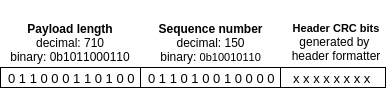
\includegraphics[width=0.6\textwidth]{img_packets/header.png}
    \caption{Example header, for a payload length of 710 bits and a packet sequence number 150. }
    \label{fig:pheader}
\end{figure}




\end{itemize}

The header format is specified in the GNU Radio Companion by adding a variable block with the following value:
\begin{minted}[frame=single,breaklines=true]{C}
digital.packet_header_default(32/constel_header.bits_per_symbol(), "packet_len", "packet_num", constel_header.bits_per_symbol())
\end{minted}
The first argument is the length of the header in symbols. In this example, \textit{constel\_header} is the constellation object that defines the header constellation. The  second argument is the name of the tag carrying the payload length. The third parameter defines which tag name the packet sequence number should get when decoding the header. The last parameter is the number of significant bits per byte at the output. A correct configuration is very important since the Extended Packet Encoder block does not repack the bytes before mapping the header bytes to symbols.
\begin{figure}[H]
    \centering
    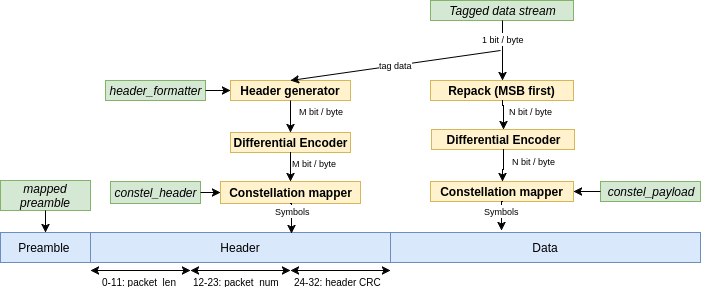
\includegraphics[width=1.05\textwidth]{img_packets/packets_flowgraph_nowhitening_diff.png}
    \caption{Schematic overview of the packet encoder implementation}
    \label{fig:packets_flowgraph}
\end{figure}
\begin{figure}[H]
    \centering
    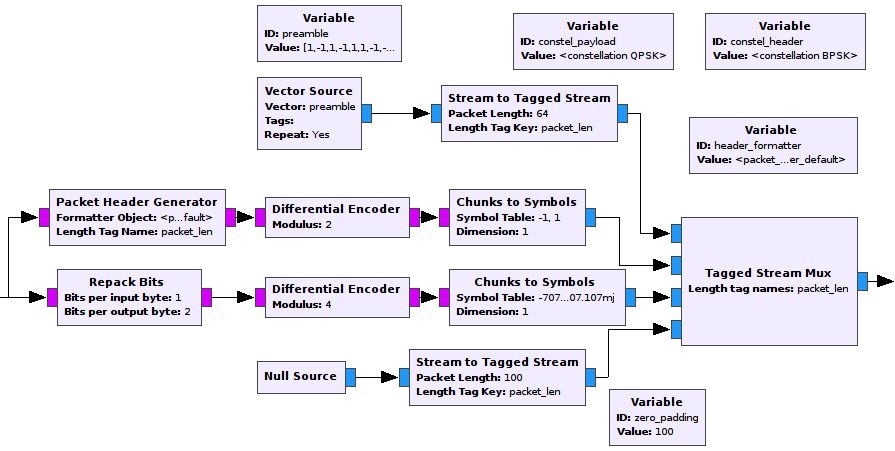
\includegraphics[width=1.05\textwidth]{img_packets/packet_enc_gr2_diff.png}
    \caption{GNU Radio Companion implementation of a packet encoder with differential encoding. Data input on the left has one bit per byte, data output on the right is one complex symbol/sample}
    \label{fig:packet_encdec}
\end{figure}




\subsubsection{Block implementation}
As described in section 2.3, a GNU Radio block can be built in C++ and Python or as a \textit{hier} block that links several existing blocks. In the packet encoder implementation as described above, many blocks do trivial operations that can be efficiently combined to eliminate the overhead of transferring data between blocks. A C++ block is the most appropriate choice.

\begin{figure}[H]
    \centering
    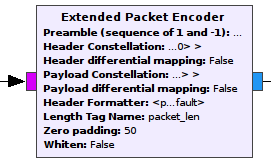
\includegraphics[width=0.45\textwidth]{img_packets/packet_enc_block.png}
    \caption{Extended Packet Encoder in the GNU Radio Companion}
    \label{fig:packet_enc_block}
\end{figure}







\subsubsection{Data example}
A simple test bench is created in order to verify the output of the implemented block. The block processes a predefined data sequence.

\begin{tight_itemize}
\item Preamble (mapped symbols): 1, -1, 1, 1
\item Payload (1 bit/byte): 0,0,0,1,0,0,1,1, \ 1,1,1,1,1,1,1,0, \  1,0,0,0,0,1,1,0, \ 0,0,1,0,1,1,1,1
\item Header mapping: \gls{bpsk} $[0,1] \rightarrow  [1, -1]$
\item Header Formatter: generated by the \textit{packet\_header\_default} class with a length of 32 bits.
\item Payload mapping: \gls{qpsk} \\$[0, 1, 2, 3] \rightarrow[-1-1j, 1-1j, -1+1j, 1+1j]$ 
\end{tight_itemize}

Output:


\begin{minted}[frame=single,breaklines=true]{C}
1,-1,-1,1,
(1+0j), (1+0j), (1+0j), (1+0j), (-1+0j), (1+0j), (1+0j), (1+0j),
(1+0j), (1+0j), (1+0j), (1+0j), (1+0j), (1+0j), (1+0j), (1+0j),
(1+0j), (1+0j), (1+0j), (1+0j), (1+0j), (1+0j), (1+0j), (1+0j),
(1+0j), (-1+0j), (-1+0j), (1+0j), (-1+0j), (-1+0j), (1+0j), (-1+0j), 
(-0.707-0.707j), (0.707-0.707j), (-0.707-0.707j), (0.707+0.707j),
(0.707+0.707j),  (0.707+0.707j), (0.707+0.707j), (-0.707+0.707j), 
(-0.707+0.707j), (-0.707-0.707j), (0.707-0.707j), (-0.707+0.707j), 
(-0.707-0.707j), (-0.707+0.707j), (0.707+0.707j), (0.707+0.707j)) 
\end{minted}

The first 4 symbols are the preamble. The next 32 symbols mapped in \gls{bpsk} have been generated for the header. When demapped to bits, this gives:
\begin{minted}[frame=single,breaklines=true]{C}
00000100 00000000 00000000 01101101
\end{minted}

The payload length in bits is stored in the first 12 bits in an LSB-first way. The decimal result is 32, which is correct. The 12 following bits encode the packet sequence number, 0 in this case. The last 8 bits are a \gls{crc} for the header.
\medskip

The \gls{qpsk} payload symbols demap to:
\begin{minted}[frame=single,breaklines=true]{C}
 00 01 00 11  | 11 11 11 10 | 10 00 01 10 | 00 10 11 11
\end{minted}
Which is the same as the input sequence.










\newpage

\subsection{Extended Packet Decoder}
\subsubsection{Requirements}
The packet decoder does the inverse operation of the packet encoder. It will demap incoming symbols to a data stream. The decoder does not know the packet length, so it should decode the header and retrieve the header length from the corresponding field. \medskip

The Extended Packet Decoder block should support the following functionality:
\begin{tight_itemize}
\item Decoding of packets that are encoded with the Extended Packet Encoder block
\item Support for both hard and soft outputs, in order to support forward error correction
\item Support for differential decoding, when hard-decision decoding is used
\end{tight_itemize}


\begin{table}[H]
\centering
\begin{tabular}{|p{6.5cm}|p{9cm}|}
\hline
 Inputs & Outputs \\ \hline
\multirow{3}{*}{
\pbox{20cm}{Complex: 1 symbol/sample \\ A tag on the incoming stream \\indicates the packet start}} &  Float: soft demapped output, samples between -1 and 1\\ \cline{2-2} 
                  &  Byte: hard demapped output with 1 bit per byte\\ \cline{2-2} 
                  & Message port: message containing header fields \\ \hline
\end{tabular}
\end{table}

\vspace*{-0.5cm}
\begin{table}[H]
\begin{center}
\begin{tabular}{|l|l|p{6cm}|}
\hline
Parameter name & Data type & Description\\
\hline
\hline

Preamble & complex vector & sequence of complex symbols for the preamble\\
\hline
Header Constellation & constellation object & pointer to the constellation object for the header\\
\hline
    Header differential mapping & boolean & use differential decoding for header data\\
\hline
Payload Constellation & constellation object & pointer to the constellation object for the payload\\
\hline
    Payload differential mapping & boolean & use differential decoding for payload data\\
\hline
Header Formatter & header formatter & pointer to the header formatter object for the header\\
\hline
Trigger Tag name & string & name of the tag that indicates the packet start and has the packet length as tag value\\
\hline
Apply Costas Loop & boolean & indicates whether phase synchronization with Costas Loop should be applied.\\
\hline
    Dewhiten & boolean & indicates whether the incoming data stream should be dewhitened.\\
    \hline
\end{tabular}
\caption{Interface of Extended Packet Decoder block}
\label{dec_interface}
\end{center}
\end{table}

\vspace*{-0.7cm}
\newpage
\subsubsection{Implementation in GNU Radio Companion}
A decoder system built in GNU Radio is shown in \reff{packet_decoder_grc}. \reff{packet_decoder_grc_diff} shows a packet decoder with differential decoding. The packet decoder is a complex block that combines several existing solutions:
\begin{tight_itemize}
\item Preamble/Header/Payload Demux: splits the input stream into a header and payload stream. In order to know the payload length, it uses the feedback loop with the decoded header data.
\item Constellation Soft Decoder: demaps symbols to soft bits.
\item Binary Slicer: maps soft bits ($-1$ and $1$) to hard bits ($0$ and $1$).
\item Tagged Stream Fix: drops unnecessary samples so packets are sequential in the stream.
\item Differential Decoder: removes the differential encoding, done in the packet encoder.
\item Packet Header Parser: decodes a header byte stream according to the header format given by the Header Formatter, which is the same one as given to the packet encoder.
\item Costas Loop: applies carrier tracking for phase synchronization, as described in section 4.3.
\end{tight_itemize}



\paragraph*{Preamble/Header/Payload Demux block}
The most important block in the decoder system is the \gls{phpd} block.
It is an extension of the existing Header/Payload Demux block, which is a highly flexible block to extract payload data with a variable length from a packet, by looking at the header fields. The block is implemented as a state machine, and one state had to be added to support preambles. The full state diagram of the \gls{phpd} block is shown in \reff{phpd}. The payload data length is given using the feedback loop for header data. Header data gets decoded and the Packet Header Parser will read the fields from the header. The result is outputted with a GNU Radio message that is forwarded to the \gls{phpd} block.\medskip 

The original Header/Payload Demux block only accepts the payload length as a number of symbols. Since the block does not know the modulation type and order, it can only split the incoming streams into a header symbol stream and payload symbol stream. \medskip

For this project, we added a new parameter called "Header Length value divider". The payload length value, received from the header, will be divided by this number and the result will be ceiled. This modification makes it possible to specify the payload length in bits, while the \gls{phpd} counts symbols.\medskip

For example, when having a payload length of 50 bits and \gls{8psk}, the packet encoder generates one zero-bit to fill all 17 symbols. The packet header carries the value 50 as \textit{packet\_len} field. The \gls{phpd} block is configured with a Header Length value divider of 3, which is the number of bits per symbol. It will calculate $ceil(50/3) = 17$ and output 17 symbols on the payload stream. The first output sample will get a tag with the name \textit{packet\_len} and value 50.\medskip

The Constellation Soft Decoder decodes each symbol to soft bits. In the case of \gls{8psk}, it outputs 3 soft bits per symbol. As a result, the output stream consists of $17\ symbols \times 3\ softbits/symbol = 51\ softbits$ which is not what the \textit{packet\_len} tag indicates. The last bit is a zero bit that is added by the packet encoder to fill the last symbol, and it should be removed from the output. The Tagged Stream Fix block will do this, as explained in the next paragraph \medskip

\begin{figure}[H]
    \centering
    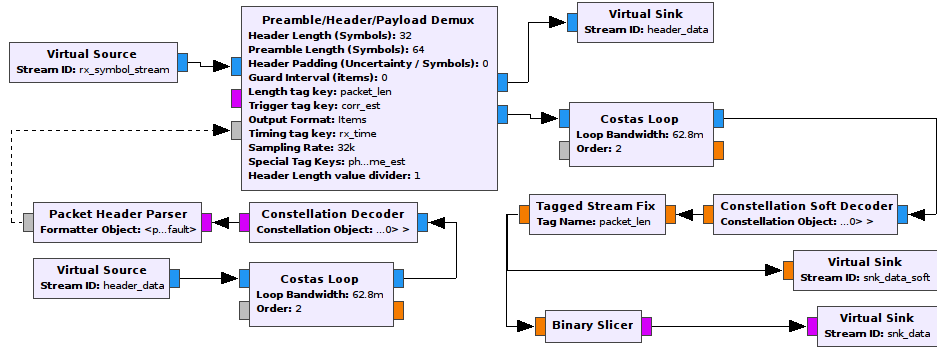
\includegraphics[width=1.05\textwidth]{img_packets/packet_decoder_grc.png}
    \caption{A packet decoder in GNU Radio Companion, configured for a \gls{bpsk} header and \gls{qpsk} payload}
    \label{fig:packet_decoder_grc}
\end{figure}

\begin{figure}[H]
    \centering
    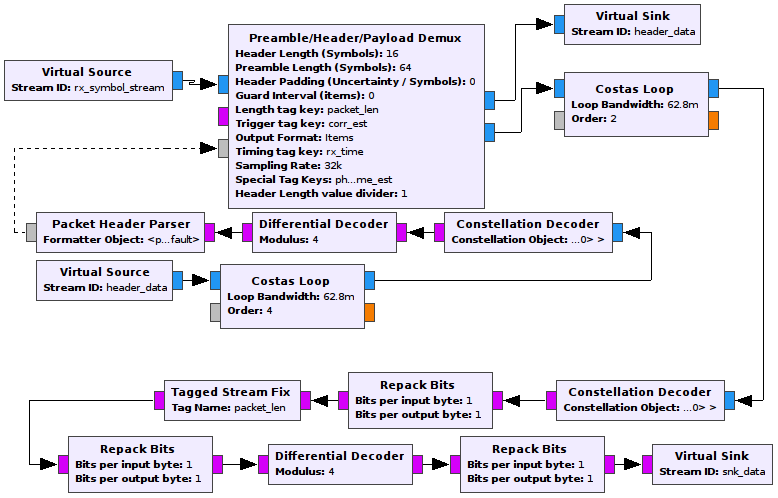
\includegraphics[width=1.0\textwidth]{img_packets/packet_decoder_grc_diff.png}
    \caption{A packet decoder in GNU Radio Companion with differential decoding, configured for a \gls{bpsk} header and \gls{qpsk} payload}
    \label{fig:packet_decoder_grc_diff}
\end{figure}






\begin{figure}[H]
    \centering
    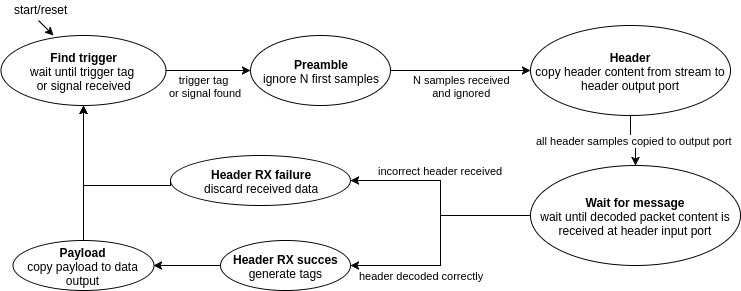
\includegraphics[width=1.05\textwidth]{img_packets/phpd.png}
    \caption{State diagram of the Preamble/Header/Payload block}
    \label{fig:phpd}
\end{figure}

\paragraph*{Tagged Stream Fix block}
A tagged stream with more samples between tags than what the \textit{packet\_len} tag indicates gives problems in GNU Radio's {tagged stream} blocks, such as the Extended Tagged FEC Decoder. These blocks expect that the packets are perfectly sequential, i.e. there are no extra samples between packets. Surprisingly, no GNU Radio block exists to remove the unnecessary samples between packets. \medskip

In this project, a block called \textit{Tagged Stream Fix} has been developed to 'truncate' a tagged data stream. 
It only keeps the samples belonging to a packet, and removes the other samples. This is illustrated in \reff{fixstream}. Because of time constraints during the project, the block is written in Python, even though a C++ block provides more throughput with less CPU usage.
\begin{figure}[H]
    \centering
    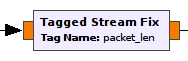
\includegraphics[width=0.3\textwidth]{img_packets/streamfix_block.png}
    \caption{Tagged Stream Fix block in GNU Radio Companion}
    \label{fig:streamfix_block}
\end{figure}
\begin{figure}[H]
    \centering
    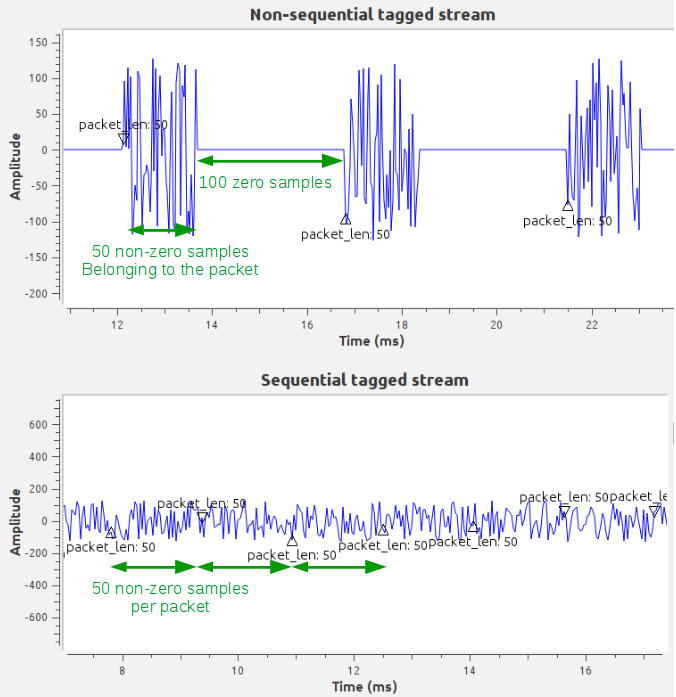
\includegraphics[width=0.9\textwidth]{img_packets/fixstream.png}
    \caption{Illustration of a non-sequential packet stream and a sequential packet stream. In the top plot, the packets are separated with zero samples, in the bottom plot the zero samples are removed.}
    \label{fig:fixstream}
\end{figure}







\subsubsection{Block implementation}
The Extended Packet Decoder block is a combination of several existing blocks, and a \textit{hier} implementation in Python is straightforward. The new block is called Extended Packet Decoder.\medskip

The header data can be analyzed by using the message output port on the Extended Packet Decoder. We developed a new block called Message Sequence Checker  to verify correct packet communication. It reads the $packet\_num$ field from the header and checks for discontinuities in packet sequence numbers. When two the difference between two sequence numbers is more than one, some packets have been dropped because they could not be detected or decoded. The block will output the number of lost packets and the packet loss rate in the console.


\begin{figure}[H]
    \centering
    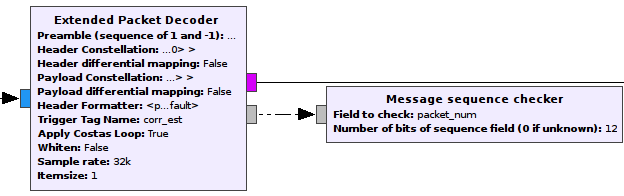
\includegraphics[width=0.8\textwidth]{img_packets/packet_dec_block.png}
    \caption{Extended Packet Encoder block and Message Sequence Checker blocks}
    \label{fig:packet_dec_block}
\end{figure}


\subsection{Packetization example systems}

\subsubsection*{Mapping}
\textit{test\_mapping.grc} is a basic example demonstrating symbol mapping and decoding. Differential encoding/decoding is also implemented.

\subsubsection*{Soft decoding}
\textit{test\_soft\_decoder.grc} illustrates the use of the {Constellation Decoder} block and the {Constellations Soft Decoder} block. An important thing to notice is that the bits should be repacked by MSB-first (instead of the default LSB-first), before mapping the bytes to symbols. The constellation receiver outputs the decoded bits MSB-first.

\subsubsection*{Prototype encoder/decoder}
\textit{encdec\_basic.grc} implements the full-featured packet encoder and decoder using basic GNU Radio blocks. \medskip

\subsubsection*{Packet encoder/decoder blocks }
\textit{encdec\_custom.grc} uses the Extended Packet Encoder/Decoder blocks, with both hard and soft demapping. \medskip